\documentclass{bioinfo}
\copyrightyear{2017}
\pubyear{2017}




%%% Additional Macro and command.
\usepackage{url}
\newcommand{\pkg}[1]{{\fontseries{b}\selectfont #1}}
\makeatletter
\newcommand\code{\bgroup\@makeother\_\@makeother\~\@makeother\$\@codex}
\def\@codex#1{{\normalfont\ttfamily\hyphenchar\font=-1 #1}\egroup}
\makeatother
\let\proglang=\textsf
%%% End of additional Macro and command.


\newcommand{\package}{\textbf{agmus }} % need that whitespace there for text flow
\usepackage{natbib}

%%% Start here.
\begin{document}


\firstpage{1}

\title[agmus]{agmus: Analyzing Genomewide Mutation and Selection pattern}
\author[
Landerer \textit{et~al}]{Cedric Landerer\,$^{1,2}$\footnote{
to whom correspondence should be addressed
},
Alexander Cope\,$^{3,5}$
Russell Zaretzki\,$^{2,4}$, and
Michael Gilchrist\,$^{1,2}$
}
\address{$^{1}$
Department of Ecology and Evolutionary Biology,
$^{2}$National Institute for Mathematical and Biological Synthesis,
$^{3}$Genome Science and Technology
$^{4}$Department of Statistics, Operations, and Management Science,
University of Tennessee, Knoxville, TN, USA,
$^{5}$Oak Ridge National Laboratory, Oak Ridge, TN, USA} 
\history{Received on XXXXX; revised on XXXXX; accepted on XXXXX}

\editor{Associate Editor: XXXXXXX}

\maketitle

\begin{abstract}

\section{Summary:}
\pkg{\package} is a fast and reliable collection of codon models, which currently estimate terms related to mutation, selection, and other population genetics parameters of interest from codon counts.
\package is fully implemented in C++ to improve computational performance and provides an ergonomic R interface for ease of use. 
\package also follows a generic object-oriented design to allow users to extend the framework and add their own models when desired.
The implemented models allow users to analyze coding sequence data and ribosome foot printing counts to estimate parameters related to ribosome overhead costs, nonsense error rates, and ribosome pausing times. 
In addition, \package features mixture distributions for parameters, allows for simulation under the provided models and implements check-pointing functionality to restart runs if necessary. 

\section{Availability:}
\pkg{\package} is freely available under the Mozilla Public License 2.0
on CRAN (\url{http://cran.r-project.org/package=agmus}).

\section{Contact:} \href{cedric.landerer@gmail.com}{cedric.landerer@gmail.com}
\end{abstract}


\section*{Introduction}
The exponential increase in publicly available genomes over the past decade and the addition of novel technologies produced a vast amount of data.  
This influx of data necessitates the development of computational tools for extracting biological information from the raw data. 
Adequate models have to be developed and provided to the public in easy to use software to allow researchers to analyze classical sequence data as well as novel data like ribosome foot-printing counts.

Here, we describe an open-source software implemented in R \citep{rcore} that allows researchers to analyze genome scale data like coding sequences and ribosome foot-printing data in a Bayesian framework under various models. 
\package implements a Gibbs sampler within a Metropolis-Hastings Monte Carlo Markov Chain (MCMC) approach which allows for the incorporation of prior knowledge and easy sampling from the posterior distribution to estimate parameter means and uncertainty.
Currently, \package provides three models to analyze codon counts obtained from coding sequences or ribosome foot-printing experiments. However, \package provides a modular infrastructure such that additional genome scale or even phylogenetic models can be integrated. 
\package provides a generic mixture distribution to all implemented models which allows for the automatic categorization of data based on differences posterior distributions for parameters of interest.

The \package framework separates data in two dimensions, e.g. genes and codons for sequence data and differentiates three types of parameters.
For all models, estimates of each type of parameter are conditioned on the other two types. 
This Gibbs sampling approach allows for a reduction in dimensionality, increasing sampling efficiency and computational performance.
1) Codon specific parameters are shared across all genes. These parameters can follow a mixture distribution and can be used to automatically or manually assign genes to clusters.
Estimation of the mixture assignment provides the probability of a gene being assigned to a mixture allowing the user to asses the uncertainty in each mixture assignment, similar to probabilistic clustering.
2) Gene specific parameters. This parameter type is estimated for each gene independently. If the codon specific parameters follow a mixture distribution, a gene specific parameter is estimated assuming the gene being assigned to each mixture. This not only solves the limitations of traditional mixture approaches but furthermore allows to test hypothesis about gene specific parameters under various conditions, represented by different mixtures.
3) Hyper parameters, like parametric prior distributions which allows for the implementation of hierarchical models.


\begin{figure*}[!tpb]
\centering
 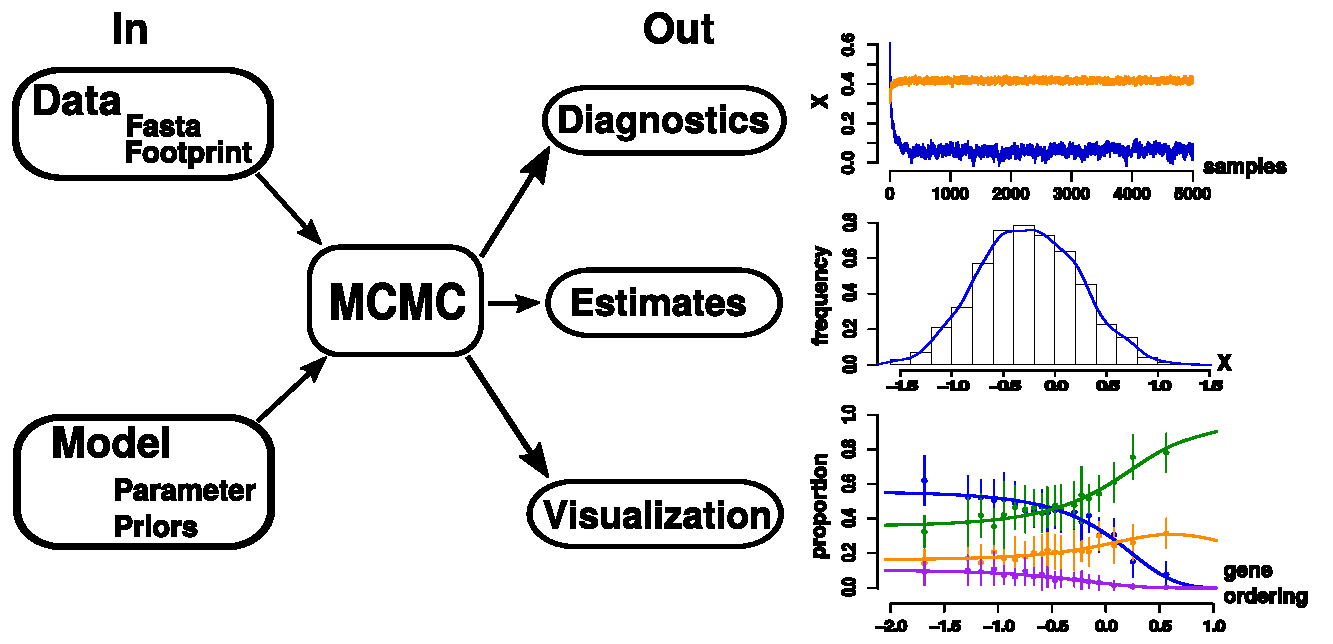
\includegraphics[width=5in]{workflow_croped.pdf}
\vspace{-0.2cm}
\caption{\textbf{Package overview and plotting functionality.} \package \textbf{Illustration of the angus workflow.} 
\package allows for the easy estimation of population genetics parameters from genome scale data such as CDS or ribosome footprints. 
Furthermore, \package provides functionality to asses goodness of fit and visualization.). 
}
\label{fig:plotbin}
\end{figure*}

\section*{Features}
\package provides an interface written in R, a freely available programming language noted for its ease of use for even inexperienced programmers. 
As a result, \package is accessible to researchers with minimal computational experience. 

\package provides a convenient interface designed to allow researchers to analyze their data swiftly without the need for long preprocessing of data sets. 
Generally, the only input needed for fitting a model to the data are protein-coding nucleotide sequences in the form of a FASTA file or a flat-file containing codon counts obtained from ribosome foot-printing experiments. 
If available, users may also provide empirically estimated values of gene expression as additional guide for the model. However, this is not required.
\package also provides visualization functionality, including plot functions to compare parameter estimates for different mixture distributions, functions to display codon usage patterns and diagnostic functions to assess the goodness of fit in a simple workflow (Figure 1).
The implemented MCMC approach automatically adapts the proposal width for sampled parameters to improve sampling efficiency and increase computational performance. 

\subsubsection*{Available models}
\package currently provides three codon models for analyzing genome scale data.
The ROC model implements the work presented by Gilchrist et al. (2015), which reliably estimates selection on \underline{r}ibosome \underline{o}verhead \underline{c}ost, mutation bias and allows for the inference of protein synthesis rates. The ROC model is an extension of work by Shah \& Gilchrist (2011) and  Wallace et al (2013). 
The NSE model is focused on the estimation of \underline{n}on-\underline{s}ense \underline{e}rror rates and accounts for the position of a codon in the sequence. Codons found later in the sequence are assumed to be under stronger selection against non-sense errors, as total energy investment is increasing along the sequence.
Both model allow for the separation of effects of mutation and selection based on gene ordering by protein synthesis rate.
Furthermore, \package implements a Pausing (PA) model to extract information on ribosome pausing times from ribosome foot-printing data. The PA model assumes that ribosome foot-print counts are inverse proportional to pausing time which is represented by a negative binomial distribution. 

%\subsubsection*{Writing extensions}
%Users are welcome and encouraged to incorporate their own codon models into \package. The object-%oriented paradigm of C++ allowed for the implementation of a general framework for creating new models %to analyze genomic data. All implemented models in \package are encapsulated such that they share %certain commonalities. This allows for the creation of new models within the same framework. Generally, %these models can be added by creating appropriate subclasses of the Parameter and Model classes provided %by the current framework. These subclasses should include the additional functionality required for %these models. 

\package defines an interface to connect all models with the implemented MCMC algorithm. 
By following this general interface, researchers are easily able to add their own models to analyze sequence and foot-printing data or novel data-types.
Researchers are able to create their own model, implementing the provided interface and inheriting functionality shared with other models.
Functionality unique to a model must be contained within the new model. 

\subsubsection*{Mixture distributions}
Mixture distributions are commonly used when a data set is comprised of sub-populations which can be described by distinguishable distributions in the parameter space \citep{gelman2013}. 
\package extends all implemented models with the ability to utilize mixture distributions for all population parameters like mutation and selection bias in the case of the ROC model. 
As all implemented model contain gene specific parameters (e.g. protein production rate) in addition to population specific parameters (e.g. mutation) we extended the mixture approach implemented in \package to incorporate the need for a gene specific parameter. 
Therefore, the protein production rate of each gene is estimated assuming it in each possible mixture distribution. 
This approach allows genes to be categorized based on differences in codon specific parameters, making \package ideal to ask questions about intra-genomic or even within-gene heterogeneity in mutation and selection patterns. 

\subsubsection*{Computational performance}
Although \package is provided as an R package, the main computational work is implemented in C++ and can be, if desired, compiled as a standalone software.
R does not provide native C++ support, but the R package Rcpp allows for the exposure of whole C++ classes as modules to R \citep{rcpp_package}.
This eliminates time consuming data transfer between the R environment and the C++ core during runs, resulting in improved computational performance and allowed for a fully object-oriented code design. 
The runtime of \package scales as expected linear with genome size and number of iterations, and polynomial with the number of mixture distributions in the data set. The polynomial increase in the number of mixture distributions is explained by the necessity to estimate the protein production rate for each gene in each mixture distribution, as it is a gene specific parameter and the probability of a gene being assigned to a mixture has to be conditioned on it.  

\bibliographystyle{natbib}
\bibliography{bioinfo}
\end{document}
